\section{Live Repository}\label{sec:lit_live} 

Literature reviews provide important information to researchers starting out in a field or practitioners who are curious to know the latest innovations, but do not have time to fully explore journals and conferences.
However, it is inevitable that a literature review such as this becomes outdated after some time, as new research comes out that cannot be included in the published paper.
This of course limits the long-term value of the work, since the text will no longer reflect the ongoing research in the field.

In order to aggregate long-term value to this work, we have made the list of papers and the information extracted from them available as an online live repository\footnote{Available at: \url{https://renangreca.github.io/literature-repository}.}.
The papers in \autoref{table:selected} serve as the starting point for a list that will continue to grow year over year.
We hope this website will serve as reference to anyone who is interested in practical applications of regression testing techniques in the coming years.

The main challenge is how to keep this repository alive in the long term.
It is unfeasible for us to add a relevant paper to the repository as soon as it is published, so our plan is to update the list in a yearly basis, re-running the query and screening steps detailed in \autoref{sec:methodology}.
That way, we can at least assure the most recent paper included is no more than one year old.
We are also looking into the possibility of getting automatic notifications when a paper that satisfies certain criteria is published in an online library.
For now, this work is done by the original authors of the literature review; according to future necessities, we will appoint other researchers or graduate students to help with the process.
In addition, we also encourage authors to submit their own work by filling a form linked on the website.

The repository also contains a separate section for relevant literature reviews.
This is initially populated by the reviews mentioned in \autoref{sec:related} and, upon publication, this very document.
With this we aim to provide a starting point for new researchers and a place to gather the overarching themes of the field.

It can also happen that, over the years, the definitions we selected for including a paper in the repository must be adjusted.
Whenever an author submits a paper, we will use the opportunity to consider whether or not the paper itself is a good fit for the repository, but also if there are new trends that our existing selection process does not account for.
There will likely be a point in the future when the industry/academia landscape has shifted and this study will no longer be needed.
When that happens, we will discuss the possibility of freezing the repository and stopping further expansions.

Aside from newer papers, it is always possible that we have missed some relevant papers for a variety of reasons, so the live repository is another way of mitigating that risk.
It is impossible to provide a complete and definitive overview of any field, but we believe that a live repository is the closest approximation that can be expected.

%\begin{figure}
%  \center
%  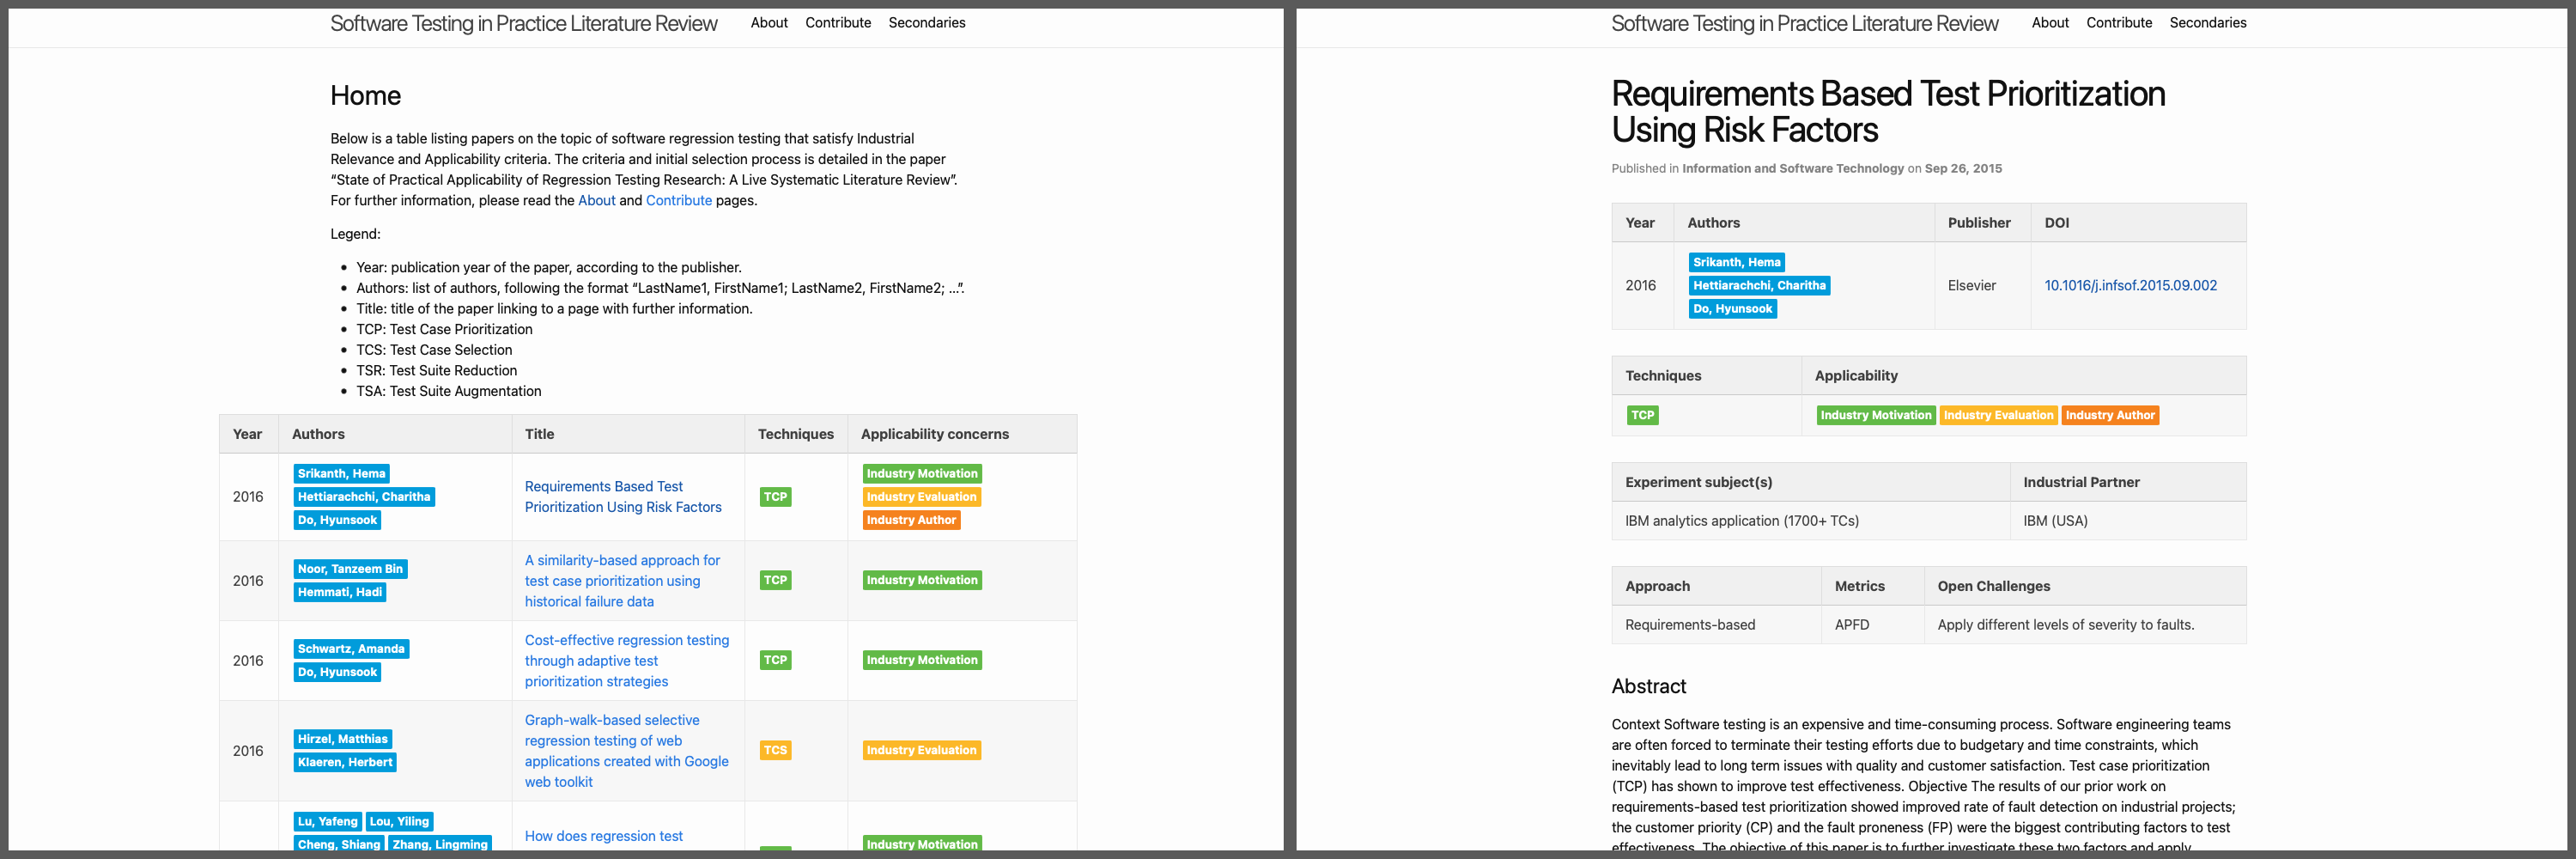
\includegraphics[width=\linewidth]{live_repository_screenshots_4.png}
%  \caption{Screenshots from the live repository. From left to right: 1) the main page listing the included papers; and 2) a single paper's page (\citetalias{srikanth_requirements_2016} used as example). }
%  \label{fig:live_repository}
%\end{figure}